% Risk heat map (Figure: risk heat map). TikZ, so it can be edited in Overleaf.
% Positions must match the L and I columns of the risk register (Table: risk). Colours follow the score
% bands in the text: L x I of 12 or more is high, 6 to 11 medium, 5 or less low.
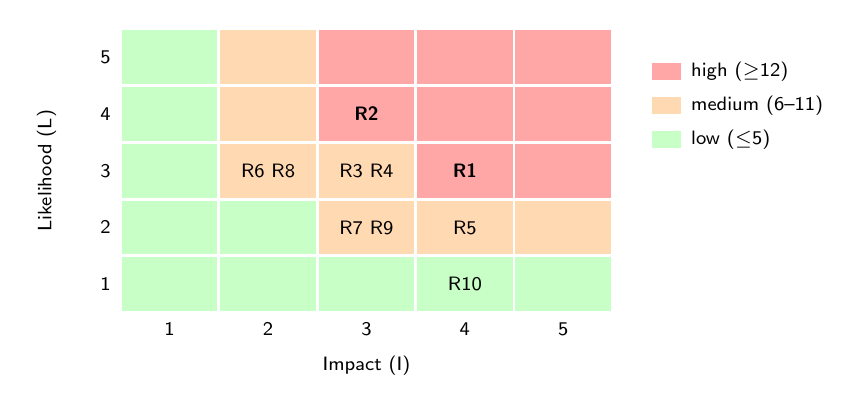
\begin{tikzpicture}[font=\sffamily\scriptsize, x=1.25cm, y=0.72cm]
  % cells, coloured by score band
  \foreach \lik in {1,...,5} {
    \foreach \imp in {1,...,5} {
      \pgfmathtruncatemacro{\score}{\lik*\imp}
      \ifnum\score>11 \def\cellcol{red!35}\else\ifnum\score>5 \def\cellcol{orange!30}\else\def\cellcol{green!22}\fi\fi
      \fill[\cellcol] (\imp-1,\lik-1) rectangle (\imp,\lik);
      \draw[white, line width=1pt] (\imp-1,\lik-1) rectangle (\imp,\lik);
    }
  }
  % axes labels
  \foreach \imp in {1,...,5} \node[below] at (\imp-0.5,0) {\imp};
  \foreach \lik in {1,...,5} \node[left] at (0,\lik-0.5) {\lik};
  \node[below=12pt] at (2.5,0) {Impact (I)};
  \node[rotate=90] at (-0.75,2.5) {Likelihood (L)};
  % risks: (impact, likelihood)
  \node at (3.5,2.5) {\textbf{R1}};          % L3 I4
  \node at (2.5,3.5) {\textbf{R2}};          % L4 I3
  \node at (2.5,2.5) {R3\,\,R4};             % L3 I3
  \node at (3.5,1.5) {R5};                   % L2 I4
  \node at (1.5,2.5) {R6\,\,R8};             % L3 I2
  \node at (2.5,1.5) {R7\,\,R9};             % L2 I3
  \node at (3.5,0.5) {R10};                  % L1 I4
  % legend
  \fill[red!35] (5.4,4.1) rectangle (5.7,4.4); \node[right] at (5.7,4.25) {high ($\geq$12)};
  \fill[orange!30] (5.4,3.5) rectangle (5.7,3.8); \node[right] at (5.7,3.65) {medium (6--11)};
  \fill[green!22] (5.4,2.9) rectangle (5.7,3.2); \node[right] at (5.7,3.05) {low ($\leq$5)};
\end{tikzpicture}
